\chapter{Problem Definition and Research Goal}
\label{chp:problem}
An overview of the problem will be given, and based on the essentials of this problem, the research goal will be discussed. It is important to define the relevance and approach to the entire research.

\section{Problem Analysis}
Due to the fourth industrial revolution, new production and manufacturing methods are required which need new digital solutions to optimize their production. One solution is \textit{centralized} analysis: combining all the data in a central database and analysing this to optimize decision making. Another solution, namely \textit{decentralisation}, analyses the data on several points, which independently create decisions.

One of the decisions for the implementation of such a system requires many considerations. Currently it is not fully clear what requirements depend on the implementation \citep{leitao2016smart}. Also, the practicality of different negotiation methods is unknown \citep{fatima2014principles}. For example, a necessity might be the requirement that the process is subject to change. If expanded or changed, many modifications in a centralized system are required since the central database has to relearn the patterns, and new databases might have to be set up. This might, however, not be the case with decentralized solutions \citep{leitao2015industrial}. %\Todo{Youri: Central is data and the management of Data insights enablers}.

A second problem is that the amount of data nowadays is enormous and as a result large quantities of data are pouring on-line, waiting to be processed in the centralized database. Furthermore, much of the data is not processed from the sensor towards the centralized database, resulting in incomplete analysis. There is an overall consensus that the future of Industry 4.0 lies with pre-aggregated data \citep{deloitte2015connected} which is obtained by having the sensors think and reason about the measurements before sending the processed information to a central database.

Thirdly, scheduling and resource allocation production problems are typical Non-deterministic Polynomial (NP)-hard problems that are very complex to solve using (mixed) integer programming and take a long time to find an optimal solution. There is a consensus that multi-agent systems retrieve a (suboptimal)-solution in reasonable time \citep{konolige1980multiple}. Since scheduling is NP-hard, this solution does not have to be the optimal solution but a ``good enough'' result.

\begin{mdframed}[style=mystyle, frametitle=IoT and CPS]

	The new developments in the industries, like the use of Internet of Things (IoT), require manufacturers to rethink their production process. An IoT is a network in which many sensors are connected using different web protocols or protocols specifically designed for IoT. These sensors retrieve their data and share the information via this network and usually communicate with a centralized database, where the data of the sensors is analysed. After analysing, production can be planned resulting in lower down time of the asset and more efficient production. When these systems are embedded, they are also known as Cyber-Physical Systems (CPS).
\end{mdframed}


\section{Area of Application}

Currently an industry leader in the production of steel is looking to optimize their de-mineralized water production. Currently their production process is done by hand, and no digital optimization method is currently in place. Furthermore, a substantial amount of some very costly materials is ``discarded'' due to legislative requirements. By using these materials instead of dumping them, cost can be reduced.

Because the main scope of this research project is aimed at negotiation, the process under consideration will undergo some idealization, meaning that it will not be too constrained. This leaves, for example, specific training levels of the mechanics out of scope. Furthermore, the possible difficult operations are excluded.  If time allows it, more constraints can be included.


\section{Relevance}%Stakeholdes=rs
The research will be relevant for two different stakeholders, the academic and business world. Business has always been dependent on the academic world, and by connecting these, new valuable insights can be combined.
\subsection{Scientific Relevance}
Currently there are not a lot of papers discussing the use of negotiation in a multi-agent solution for manufacturing. There are comprehensive overviews of agent-based manufacturing, but the negotiation aspect is a commonly lacking subject \citep{leitao2009agent}. In \Cref{ch:literature} a comprehensive overview will be given. By researching and, importantly, computationally implementing the use of negotiation in distributed production planning, the theory can be connected to real life cases. This is based on the classic artificial intelligence problem, which is the combination of information and objectives from different sources and will be solved by the way of a multi-agent system.

This research is about the application of multi-agent system technology, negotiation, game theory and decision making. Knowledge from artificial intelligence about negotiation will be used to obtain new insights in possible decentralized production solutions.

For me personally this research project would be a perfect way to find out how ideas and solutions in the AI literature can be used to describe and improve large-scale and real-world solutions.
\subsection{Business Relevance}
The business has difficulty in the transformation to the new industrial pillars. Enormous amounts of data and new requirements require ``on top of the line'' production systems. By computationally implementing one of the processes and optimizing these processes, these insights can be applied for further use. An obvious solution lies in Multi-Agent Systems, but the exact implementation is difficult.

Furthermore, the insights of negotiation are very useful in every aspect of a business. A little more knowledge on how to optimize one's negotiation helps optimize your business professionally.
\section{Research Goal}
The main goal is to optimize a process using a multi-agent system with negotiation. This is divided into the following sub-goals:
\begin{enumerate}
	\item
	Provide a theoretical framework for negotiation in a multi-agent system in the context of manufacturing \& production.
	\item
	Create a simulator to show that a multi-agent system can be used for manufacturing/production planning.
	\item
	Determine what steps are necessary for a business to make use of negotiation in such a new multi-agent system. 
\end{enumerate} 


\section{Research Approach}
\label{sec:researchapproach}
Since this is an academic research project, a new MAS framework will be investigated and constructed. The working and exact results will be analysed by the use of a demonstrator. This falls under the computational implementation and modelling of a new MAS framework. This excludes the verification (use users to control your theory) and validation of the system.

The research framework used will be based on \citep{hevner2010design} and can be seen in \Cref{fig:InformationSystemResearchFramework}. The aim of the relevance cycle is to connect the real-world environment of the research project with the design science activities. Through this relevance cycle, opportunities for the improvement of practices can be identified.

The rigor cycle is used to assemble a knowledge base that consists of the relevant theoretical foundations and research methodologies. Prior research provides a starting point and benchmark for new artefacts. This knowledge base is necessary to establish theoretical appropriateness and relevance, achieving rigor.

\begin{figure}[h]
	\centering
	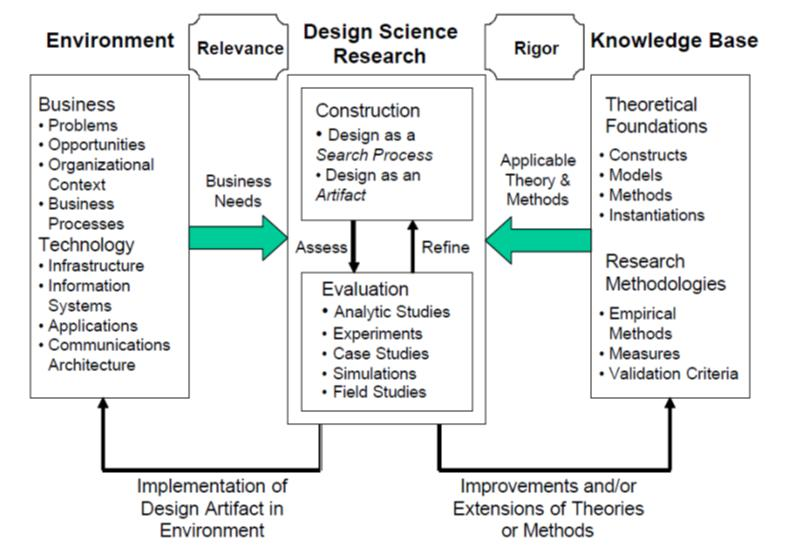
\includegraphics[width=0.7\linewidth]{./img/InformationSystemResearchFramework.jpg}
	\caption{The Information System Research Framework as designed by \citet{hevner2010design}}
	\label{fig:InformationSystemResearchFramework}
\end{figure}

In this research, a case-study is done to check the working of negotiation in this new MAS framework. By comparing the model with a real-world situation, the new MAS framework can be assessed and maybe refined. Furthermore, it can be determined whether this negotiation method can be used in a business context.

\section{Research Process}
Firstly a literature research was concluded to assess agent-based solution in the manufacturing world. Furthermore, the current negotiation methods in agent solutions were reviewed. From the literature a knowledge gap was found, which could used in future manufacturing processes. Based on this knowledge gap, a mathematical model was created, to assess how the negotiation will concur in the multi-agent system. A simulator was created to evaluate this method. After the creation of the model and simulator, the relevance was assessed by its performance.

\subsection{Evaluation Method}
To test the final theoretical framework, a virtual simulation is created. By having the agents negotiate regarding the optimal resource allocation, and by using different negotiation methods, it can be shown that negotiation can be applied to find a possible (near-) optimal outcome. The model is to be evaluated using the known Nash solution. Since all the utilities are known, the optimal solution of the group can be determined. From this the effectivity of the method, and an evaluation of the model in aspects of speed, quality solution, and dynamicity can be made.

\section{Research Questions}
From the research goals and process, the following research questions are concluded:
\begin{enumerate}
	\item
	How can energy and manufacturing companies use the AI concept of intelligent multi-agent systems (MAS) for the optimization of production planning incl predictive maintenance and/or process control optimization?
	\begin{enumerate}
		\item
		What is the optimal MAS framework for the optimization of production planning?
		\begin{enumerate}
			\item 
			Theoretical: Which negotiation techniques, communication protocols, knowledge models and hierarchy/coalition can be used to optimize decision making for production processes?
			\item
			Simulation: How does this new framework compare using an existing use case using simulation results?
		\end{enumerate}
		\item
		What is the general framework within the Industry 4.0?
		\begin{enumerate}
			\item 
			What is the difference between a decentralized systems and a centralized system?
			\item
			How can negotiation be used in manufacturing?
		\end{enumerate}
	\end{enumerate}
\end{enumerate}

